\documentclass[11pt,a4paper]{article}
\usepackage[utf8]{inputenc}
\usepackage[vietnamese]{babel}
\usepackage{amsmath,amssymb}
\usepackage[version=4]{mhchem}
\usepackage{geometry}
\geometry{top=1.5cm,bottom=1.2cm,left=1.4cm,right=1.4cm,headheight=28pt,headsep=12pt,footskip=18pt}
\usepackage{graphicx}
\usepackage{xcolor}
\usepackage{tabularx}
\usepackage{array}
\usepackage{colortbl}
\usepackage{tikz}
\usepackage{fancyhdr}
\usepackage{enumitem}

\graphicspath{{images_quangtrung2_hoa12_2102/}{San_Pham/images_quangtrung2_hoa12_2102/}{C:/Antigravity_Thanh/San_Pham/images_quangtrung2_hoa12_2102/}}

\definecolor{hfRed}{HTML}{D32F2F}
\definecolor{hfGreen}{HTML}{8BC390}
\definecolor{mainGreen}{HTML}{2E7D32}
\definecolor{solBlue}{HTML}{1565C0}
\definecolor{tableGreen}{HTML}{E8F5E9}

\usepackage{ex_test}

\pagestyle{fancy}
\fancyhf{}
\renewcommand{\headrulewidth}{0.75pt}
\renewcommand{\headrule}{\hbox to\headwidth{\color{hfGreen}\leaders\hrule height \headrulewidth\hfill}}
\renewcommand{\footrulewidth}{0.75pt}
\renewcommand{\footrule}{\hbox to\headwidth{\color{hfGreen}\leaders\hrule height \footrulewidth\hfill}}

\fancyhead[L]{\small\itshape\color{hfRed}Tài liệu lưu hành nội bộ}
\fancyhead[R]{\small\color{hfRed}Thầy \textbf{TRẦN VĂN THẠNH} - 0777.470.803}

\fancyfoot[L]{\footnotesize\itshape\color{hfRed}CS1: 6/15 Nguyễn Hoàng, P. Kim Long, TP Huế \quad|\quad CS2: 24 Đặng Thái Thân, TP Huế}
\fancyfoot[R]{\small\textbf{\color{hfRed}Trang \thepage}}

\setlength{\parindent}{0pt}
\setlength{\parskip}{2pt}

\begin{document}


\noindent
\begin{minipage}[t]{0.48\textwidth}
\textbf{SỞ GD \& ĐT GIA LAI}\\
\textbf{TRƯỜNG THPT SỐ 2 QUANG TRUNG}\\
\textbf{ĐỀ CHÍNH THỨC}\\
\textit{(Đề thi có 04 trang)}
\end{minipage}
\hfill
\begin{minipage}[t]{0.48\textwidth}
\raggedleft
\textbf{\color{hfRed}ĐỀ KIỂM TRA GIỮA KỲ I, NĂM HỌC 2026 - 2027}\\
\textbf{MÔN: HÓA HỌC -- KHỐI 12}\\
\textit{Thời gian làm bài: 45 phút (không kể thời gian phát đề)}\\
\textbf{MÃ ĐỀ: 2102}
\end{minipage}

\vspace{4pt}
\noindent
\textit{Họ và tên thí sinh:} \dotfill \textit{Lớp:} \dots\dots\dots \textit{Số báo danh:} \dotfill

\vspace{3pt}
\noindent
\textit{\footnotesize Cho nguyên tử khối của các nguyên tố: C = 12; H = 1; O = 16; Na = 23; Br = 80; N = 14.}

\vspace{2pt}
\hrule height 0.5pt


\vspace{6pt}
\noindent
{\color{mainGreen}\textbf{\large PHẦN I. CÂU TRẮC NGHIỆM NHIỀU PHƯƠNG ÁN LỰA CHỌN (4,0 điểm)}}

\textit{Thí sinh trả lời từ câu 1 đến câu 16. Mỗi câu hỏi thí sinh chỉ chọn một phương án.}

\vspace{2pt}


\begin{ex}
Cho các phát biểu sau:
\begin{enumerate}[label=(\arabic*),itemsep=1pt,leftmargin=1.8cm]
\item Alkylamine bậc một tác dụng với nitrous acid ở nhiệt độ thường tạo alcohol và giải phóng khí nitrogen.
\item Dung dịch methylamine tác dụng với dung dịch $\ce{FeCl3}$ tạo kết tủa nâu đỏ $\ce{Fe(OH)3}$.
\item Tripeptide Ala-Gly-Ala tham gia phản ứng màu biuret.
\item Ở điều kiện thường, các amino acid là chất lỏng, ít tan trong nước.
\item Protein trong dung dịch lòng trắng trứng bị đông tụ khi đun nóng.
\item Aniline dễ tham gia phản ứng thế nguyên tử hydrogen ở nhân thơm hơn benzene.
\end{enumerate}
Số phát biểu đúng là
\choice
{\True 5}
{4}
{2}
{3}

\end{ex}

\begin{ex}
Mùi tanh của cá chủ yếu do trimethylamine gây ra. Phát biểu nào sau đây \textbf{đúng} về tính chất vật lí của amine?
\choice
{Các amine có số nguyên tử carbon nhỏ đều không tan trong nước}
{\True Trimethylamine là chất khí ở điều kiện thường}
{Tất cả các amine đều là chất rắn ở điều kiện thường}
{Aniline là chất khí, tan tốt trong nước}

\end{ex}

\begin{ex}
Dãy nào sau đây gồm polysaccharide?
\choice
{\True Tinh bột, cellulose}
{Saccharose, maltose}
{Glucose, fructose}
{Glucose, saccharose}

\end{ex}

\begin{ex}
Saccharose được dùng nhiều trong sản xuất bánh kẹo và nước giải khát. Saccharose có nhiều trong
\choice
{hạt gạo và hạt ngô}
{gỗ và sợi bông}
{\True cây mía, củ cải đường và hoa thốt nốt}
{hạt đang nảy mầm}

\end{ex}

\begin{ex}
Amine $\ce{CH3NHCH3}$ có tên gốc - chức là
\choice
{\True dimethylamine}
{methylamine}
{trimethylamine}
{ethylamine}

\end{ex}

\begin{ex}
Ở $\text{pH} = 2$, khi đặt dung dịch glycine trong điện trường thì glycine di chuyển về phía
\choice
{cực dương (+)}
{không di chuyển}
{\True cực âm (--)}
{cả hai cực}

\end{ex}

\begin{ex}
Ester $\ce{CH3CH2COOCH3}$ có tên gọi là
\choice
{methyl ethanoate}
{\True methyl propanoate}
{ethyl ethanoate}
{propyl methanoate}

\end{ex}

\begin{ex}
Mỡ lợn, dầu lạc, dầu hướng dương là những nguồn cung cấp chất béo quen thuộc trong bữa ăn hằng ngày. Về cấu tạo, chất béo là
\choice
{ester của glycerol với acid vô cơ}
{monoester của glycerol với acid béo}
{\True triester của glycerol với acid béo}
{diester của glycerol với acid béo}

\end{ex}

\begin{ex}
Dung dịch saccharose không phản ứng với thuốc thử Tollens. Đun nóng dung dịch saccharose với dung dịch $\ce{H2SO4}$ loãng, để nguội rồi trung hòa acid dư bằng dung dịch $\ce{NaOH}$. Thêm thuốc thử Tollens vào dung dịch sau xử lí và đun cách thủy, thấy xuất hiện bạc. Nguyên nhân là do:
\choice
{\True saccharose bị thủy phân tạo thành glucose và fructose, các sản phẩm này phản ứng được với thuốc thử Tollens}
{trong dung dịch, saccharose tồn tại chủ yếu ở dạng mạch hở có nhóm $\ce{-CHO}$}
{acid loãng oxi hóa saccharose thành các chất có nhóm $\ce{-CHO}$}
{acid loãng khử ion $\ce{Ag+}$ trong thuốc thử Tollens thành $\ce{Ag}$}

\end{ex}

\begin{ex}
Chất nào sau đây là amine bậc hai?
\choice
{\True $\ce{CH3NHC2H5}$}
{$\ce{(CH3)3N}$}
{$\ce{CH3NH2}$}
{$\ce{C6H5NH2}$}

\end{ex}

\begin{ex}
Ethyl butanoate và ethyl ethanoate là những ester có mùi thơm, được dùng làm chất tạo hương trong công nghiệp thực phẩm và mĩ phẩm. Khi thay thế nhóm $\ce{-OH}$ trong nhóm carboxyl ($\ce{-COOH}$) của carboxylic acid bằng nhóm $-\ce{OR}'$ ($\text{R}'$ là gốc hydrocarbon) thì thu được hợp chất thuộc loại nào sau đây?
\choice
{Amino acid}
{Alcohol}
{Amine}
{\True Ester}

\end{ex}

\begin{ex}
Một cơ sở tận dụng dầu ăn đã qua sử dụng để sản xuất biodiesel. Trong quy trình tái chế, chất béo trong dầu ăn phản ứng với methanol có xúc tác thích hợp, tạo các methyl ester của acid béo và glycerol theo phương trình tổng quát sau:
\[ \ce{(RCOO)3C3H5 + 3CH3OH ->[\text{xúc tác},\, t^\circ] 3RCOOCH3 + C3H5(OH)3} \]
Cơ sở sử dụng $100\text{ kg}$ dầu ăn đã qua sử dụng chứa $88{,}4\%$ triolein theo khối lượng, phần còn lại là tạp chất không tham gia phản ứng và không tạo biodiesel. Cho lượng dầu này phản ứng với methanol dư, hiệu suất chuyển hóa triolein thành methyl oleate đạt $90\%$. Khối lượng biodiesel thu được là bao nhiêu, biết biodiesel trong bài toán chỉ gồm methyl oleate?
\choice
{\True $79{,}92\text{ kg}$}
{$79{,}56\text{ kg}$}
{$88{,}80\text{ kg}$}
{$26{,}64\text{ kg}$}

\end{ex}

\begin{ex}
Trong sản xuất thực phẩm, dầu thực vật có thể được chế biến thành chất béo có độ rắn cao hơn, dùng làm nguyên liệu sản xuất bơ thực vật. Quá trình hóa học nào sau đây giúp thực hiện sự chuyển đổi này?
\choice
{\True Chất béo lỏng chứa gốc acid béo không no cộng $\ce{H2}$ (có xúc tác, nhiệt độ thích hợp) tạo thành chất béo chứa gốc acid béo no ở dạng rắn}
{Thủy phân chất béo trong dầu thực vật thành glycerol và acid béo}
{Xà phòng hóa chất béo trong dầu thực vật bằng dung dịch $\ce{NaOH}$}
{Oxi hóa chất béo trong dầu thực vật bằng oxygen không khí}

\end{ex}

\begin{ex}
Dung dịch glucose $5\%$ được dùng để truyền tĩnh mạch nhằm cung cấp năng lượng nhanh cho bệnh nhân. Glucose thuộc loại carbohydrate nào sau đây?
\choice
{Disaccharide}
{Lipid}
{Polysaccharide}
{\True Monosaccharide}

\end{ex}

\begin{ex}
Ethanol sinh học (cồn sinh học) được dùng làm nhiên liệu sinh học, được sản xuất bằng cách lên men các nguyên liệu chứa tinh bột. Từ 1 tấn sắn khô chứa $81\%$ tinh bột về khối lượng, với hiệu suất của toàn bộ quá trình là $70\%$, khối lượng ethanol thu được là
\choice
{$230\text{ kg}$}
{$414\text{ kg}$}
{\True $322\text{ kg}$}
{$460\text{ kg}$}

\end{ex}

\begin{ex}
Tiến hành thí nghiệm như hình vẽ sau: nhỏ một giọt dung dịch methylamine $0{,}1\text{ M}$ lên mẩu giấy quỳ tím đặt trên mặt kính đồng hồ (1), nhỏ một giọt dung dịch aniline $0{,}1\text{ M}$ lên mẩu giấy quỳ tím đặt trên mặt kính đồng hồ (2).
\begin{center}
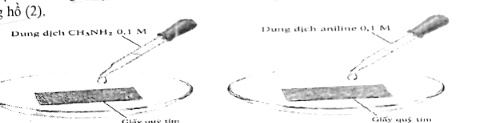
\includegraphics[width=11cm]{images_quangtrung2_hoa12_2102/hinh_cau16_quy_tim.png}
\end{center}
Hiện tượng quan sát được là
\choice
{cả hai mẩu giấy quỳ tím đều chuyển sang màu xanh}
{\True giấy quỳ tím (1) chuyển sang màu xanh, giấy quỳ tím (2) không đổi màu}
{giấy quỳ tím (1) không đổi màu, giấy quỳ tím (2) chuyển sang màu xanh}
{cả hai mẩu giấy quỳ tím đều không đổi màu}

\end{ex}

\vspace{6pt}
\noindent
{\color{mainGreen}\textbf{\large PHẦN II. CÂU TRẮC NGHIỆM ĐÚNG SAI (2,0 điểm)}}

\textit{Thí sinh trả lời từ câu 1 đến câu 2. Trong mỗi ý a), b), c), d) ở mỗi câu, thí sinh chọn đúng hoặc sai.}

\vspace{2pt}


\begin{ex}
Tinh bột có nhiều trong gạo, ngô, khoai; cellulose là thành phần chính của sợi bông và có trong gỗ. Hai chất này có vai trò quan trọng trong đời sống nhưng khác nhau về cấu tạo và tính chất. Hãy xác định các phát biểu sau là đúng hay sai:
\choiceTF
{Tinh bột và cellulose đều là polysaccharide có công thức tổng quát $\ce{(C6H10O5)_n}$ nên có cấu tạo hoàn toàn giống nhau.}
{\True Trong cơ thể người, tinh bột được thủy phân qua các sản phẩm trung gian, cuối cùng tạo glucose. Glucose được hấp thu vào máu, cung cấp năng lượng hoặc chuyển thành glycogen dự trữ.}
{Tinh bột là chất rắn màu trắng, tan tốt trong nước lạnh.}
{Hồ tinh bột đã trộn với dung dịch iodine mất màu khi đun nóng nhẹ và xuất hiện lại màu xanh tím khi để nguội vì tinh bột đã thủy phân hoàn toàn thành glucose.}

\end{ex}

\begin{ex}
Một nhóm học sinh tìm hiểu tính chất của protein trong lòng trắng trứng bằng thí nghiệm được mô tả trong hình dưới đây, kết quả thu được dung dịch X.
\begin{center}
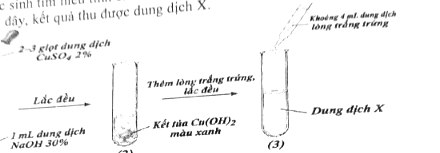
\includegraphics[width=12cm]{images_quangtrung2_hoa12_2102/hinh_p2_cau2_biuret.png}
\end{center}
Hãy xác định các phát biểu sau là đúng hay sai:
\choiceTF
{Nếu thay dung dịch lòng trắng trứng bằng dung dịch glycine thì vẫn xuất hiện màu tím đặc trưng của phản ứng biuret.}
{\True Các protein dạng hình sợi như keratin (trong tóc, móng), collagen (trong da, sụn) không tan trong nước.}
{\True Dung dịch X có màu tím.}
{\True Khi nấu ăn người ta dùng nước ép dứa tươi để làm mềm thịt vì enzyme bromelain trong nước ép dứa tươi có khả năng xúc tác phản ứng thủy phân protein.}

\end{ex}

\vspace{6pt}
\noindent
{\color{mainGreen}\textbf{\large PHẦN III. CÂU TRẮC NGHIỆM TRẢ LỜI NGẮN (2,0 điểm)}}

\textit{Thí sinh trả lời từ câu 1 đến câu 4. Điền kết quả trả lời vào phiếu làm bài.}

\vspace{2pt}


\begin{ex}
Saccharose được dùng phổ biến làm đường ăn, còn maltose có trong sản phẩm thủy phân tinh bột. Xét các đặc điểm cấu tạo sau:
\begin{enumerate}[label=(\arabic*),itemsep=1pt,leftmargin=1.8cm]
\item Trong cấu tạo phân tử có hai đơn vị monosaccharide liên kết với nhau.
\item Có 8 nhóm $\ce{-OH}$ trong phân tử.
\item Chỉ được tạo thành từ các đơn vị glucose.
\item Có 1 nhóm $\ce{-OH}$ hemiacetal tự do.
\end{enumerate}
Có bao nhiêu đặc điểm đúng với cả saccharose và maltose ở dạng vòng?


\par\noindent\textbf{Trả lời:} \dotfill

\end{ex}

\begin{ex}
Xà phòng và chất giặt rửa tổng hợp được sử dụng phổ biến trong đời sống. Xét các phát biểu sau về phương pháp sản xuất và cách sử dụng hai loại sản phẩm này:
\begin{enumerate}[label=\alph*),itemsep=1pt,leftmargin=1.5cm]
\item Xà phòng có thể được sản xuất bằng cách đun nóng chất béo với dung dịch $\ce{NaOH}$ hoặc $\ce{KOH}$.
\item Phương pháp chủ yếu để sản xuất chất giặt rửa tổng hợp là đun nóng chất béo với dung dịch kiềm.
\item Trong sản xuất chất giặt rửa tổng hợp, có thể sulfo hoá alkylbenzene rồi trung hoà sản phẩm bằng $\ce{NaOH}$ để thu được sodium alkylbenzenesulfonate.
\item Khi giặt bằng nước cứng, xà phòng tạo kết tủa với ion $\ce{Ca^2+}$, $\ce{Mg^2+}$ nên bị giảm tác dụng giặt rửa.
\item Cần sử dụng xà phòng và chất giặt rửa tổng hợp đúng mục đích, đúng liều lượng theo hướng dẫn, tránh để sản phẩm tiếp xúc với mắt.
\end{enumerate}
Có bao nhiêu phát biểu đúng?


\par\noindent\textbf{Trả lời:} \dotfill

\end{ex}

\begin{ex}
Cho $\ce{Cu(OH)2}$ mới tạo vào dung dịch Gly-Ala-Gly trong môi trường kiềm, lắc đều thấy xuất hiện màu tím. Xét các nhận định:
\begin{enumerate}[label=(\arabic*),itemsep=1pt,leftmargin=1.8cm]
\item Gly-Ala-Gly có hai liên kết peptide trong phân tử.
\item Màu tím xuất hiện do peptide tạo phức với ion $\ce{Cu^2+}$ trong môi trường kiềm.
\item Thay Gly-Ala-Gly bằng Gly-Ala vẫn thu được màu tím đặc trưng tương tự.
\item Sau khi thuỷ phân hoàn toàn Gly-Ala-Gly, hỗn hợp sản phẩm không còn cho phản ứng màu biuret.
\end{enumerate}
Có bao nhiêu nhận định đúng?


\par\noindent\textbf{Trả lời:} \dotfill

\end{ex}

\begin{ex}
Tiến hành thí nghiệm nhỏ aniline loãng vào nước bromine dư như hình sau:
\begin{center}
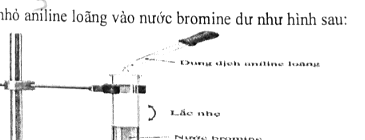
\includegraphics[width=9cm]{images_quangtrung2_hoa12_2102/hinh_p3_cau4_aniline_bromine.png}
\end{center}
Xét các nhận định:
\begin{enumerate}[label=(\arabic*),itemsep=1pt,leftmargin=1.8cm]
\item Xuất hiện kết tủa trắng là 2,4,6-tribromoaniline.
\item Do ảnh hưởng của nhóm $\ce{-NH2}$ lên vòng benzene nên aniline tham gia phản ứng thế nguyên tử hydrogen dễ hơn benzene.
\item Nếu thay dung dịch aniline trong thí nghiệm trên bằng dung dịch alanine thì vẫn thu được kết tủa trắng.
\item Cho $0{,}01\text{ mol}$ aniline phản ứng hoàn toàn với nước bromine dư thì thấy $4{,}8\text{ gam}$ bromine phản ứng.
\end{enumerate}
Có bao nhiêu nhận định đúng?


\par\noindent\textbf{Trả lời:} \dotfill

\end{ex}

\vspace{6pt}
\noindent
{\color{mainGreen}\textbf{\large PHẦN IV. TỰ LUẬN (2,0 điểm)}}

\textit{Thí sinh trả lời từ câu 1 đến câu 2. Trình bày chi tiết lời giải vào giấy làm bài thi.}

\vspace{2pt}


\begin{ex}
\textbf{(1,0 điểm)} Để tìm hiểu tính chất hóa học của glucose tiến hành thí nghiệm như sau:
\begin{itemize}[leftmargin=*,itemsep=1pt]
\item \textit{Bước 1:} Cho vào mỗi ống nghiệm (1) và (2) lần lượt $3\text{ mL}$ dung dịch $\ce{NaOH}\ 10\%$, $0{,}6\text{ mL}$ dung dịch $\ce{CuSO4}\ 5\%$ rồi lắc đều. Tiếp tục thêm vào mỗi ống $3\text{ mL}$ dung dịch glucose $5\%$ và lắc đều.
\item \textit{Bước 2:} Giữ ống nghiệm (1) ở nhiệt độ thường, đun nóng nhẹ ống nghiệm (2) bằng đèn cồn trong vài phút. Cách bố trí thí nghiệm được mô tả trong hình.
\end{itemize}
\begin{center}
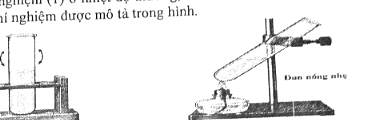
\includegraphics[width=12cm]{images_quangtrung2_hoa12_2102/hinh_p4_cau1_glucose_cuoh2.png}
\end{center}
a) \textit{(0,5 điểm)} Nêu hiện tượng quan sát được ở mỗi ống nghiệm. Mỗi hiện tượng đó chứng tỏ trong phân tử glucose có nhóm chức nào?\\
b) \textit{(0,5 điểm)} Viết phương trình hóa học của phản ứng xảy ra ở ống nghiệm (2).


\vspace{5cm}

\end{ex}

\begin{ex}
\textbf{(1,0 điểm)} Trong phòng thí nghiệm, một nhóm học sinh tiến hành thí nghiệm cho tristearin tác dụng với dung dịch $\ce{NaOH}$ và xử lí sản phẩm theo quy trình minh họa dưới đây để tạo xà phòng (sản phẩm mang tính thực nghiệm và chưa được đánh giá chất lượng sử dụng):
\begin{center}
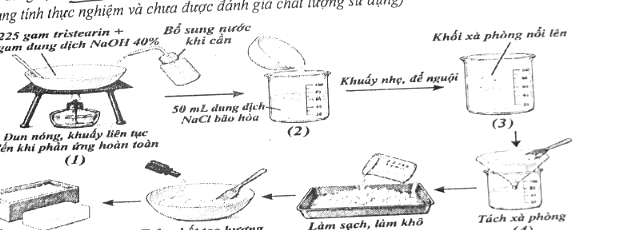
\includegraphics[width=14cm]{images_quangtrung2_hoa12_2102/hinh_p4_cau2_quy_trinh_xa_phong.png}
\end{center}
a) \textit{(0,25 điểm)} Viết phương trình hóa học của phản ứng xà phòng hóa tristearin bằng $\ce{NaOH}$.\\
b) \textit{(0,25 điểm)} Nêu vai trò của dung dịch $\ce{NaCl}$ bão hòa ở giai đoạn (2) trong thí nghiệm.\\
c) \textit{(0,5 điểm)} Một cơ sở sản xuất nhận đơn hàng gồm 48 bánh xà phòng, mỗi bánh có khối lượng $80\text{ gam}$, trong đó sodium stearate chiếm $76{,}5\%$ khối lượng, phần còn lại là các chất phụ gia. Cơ sở sử dụng tristearin nguyên chất phản ứng hoàn toàn với $\ce{NaOH}$ dư. Do hao hụt trong quá trình tách và xử lí sản phẩm, khối lượng sodium stearate thực tế thu được bằng $80\%$ khối lượng tính theo lí thuyết. Tính khối lượng tristearin tối thiểu cần dùng để hoàn thành đơn hàng, theo đơn vị kg.


\vspace{6cm}

\end{ex}

\vspace{8pt}
\begin{center}
\textbf{---------- HẾT ----------}
\end{center}

\end{document}
